\documentclass{article}
\usepackage[utf8]{inputenc}
\usepackage{graphicx}   % Include PNG/JPG
\usepackage{caption}    % Better captions
\usepackage{float}      % [H] placement

\title{Drone Project Figures}
\author{Samuel Tadamatla and Evan Phillips}
\date{\today}

\begin{document}
	
	\maketitle
	
	\section{Introduction}
	This document compiles all drone setup images and data figures from the project.
	
	\section{Drone Setup Images}
	
	% Figure 1: Drone photo
	\begin{figure}[H]
		\centering
		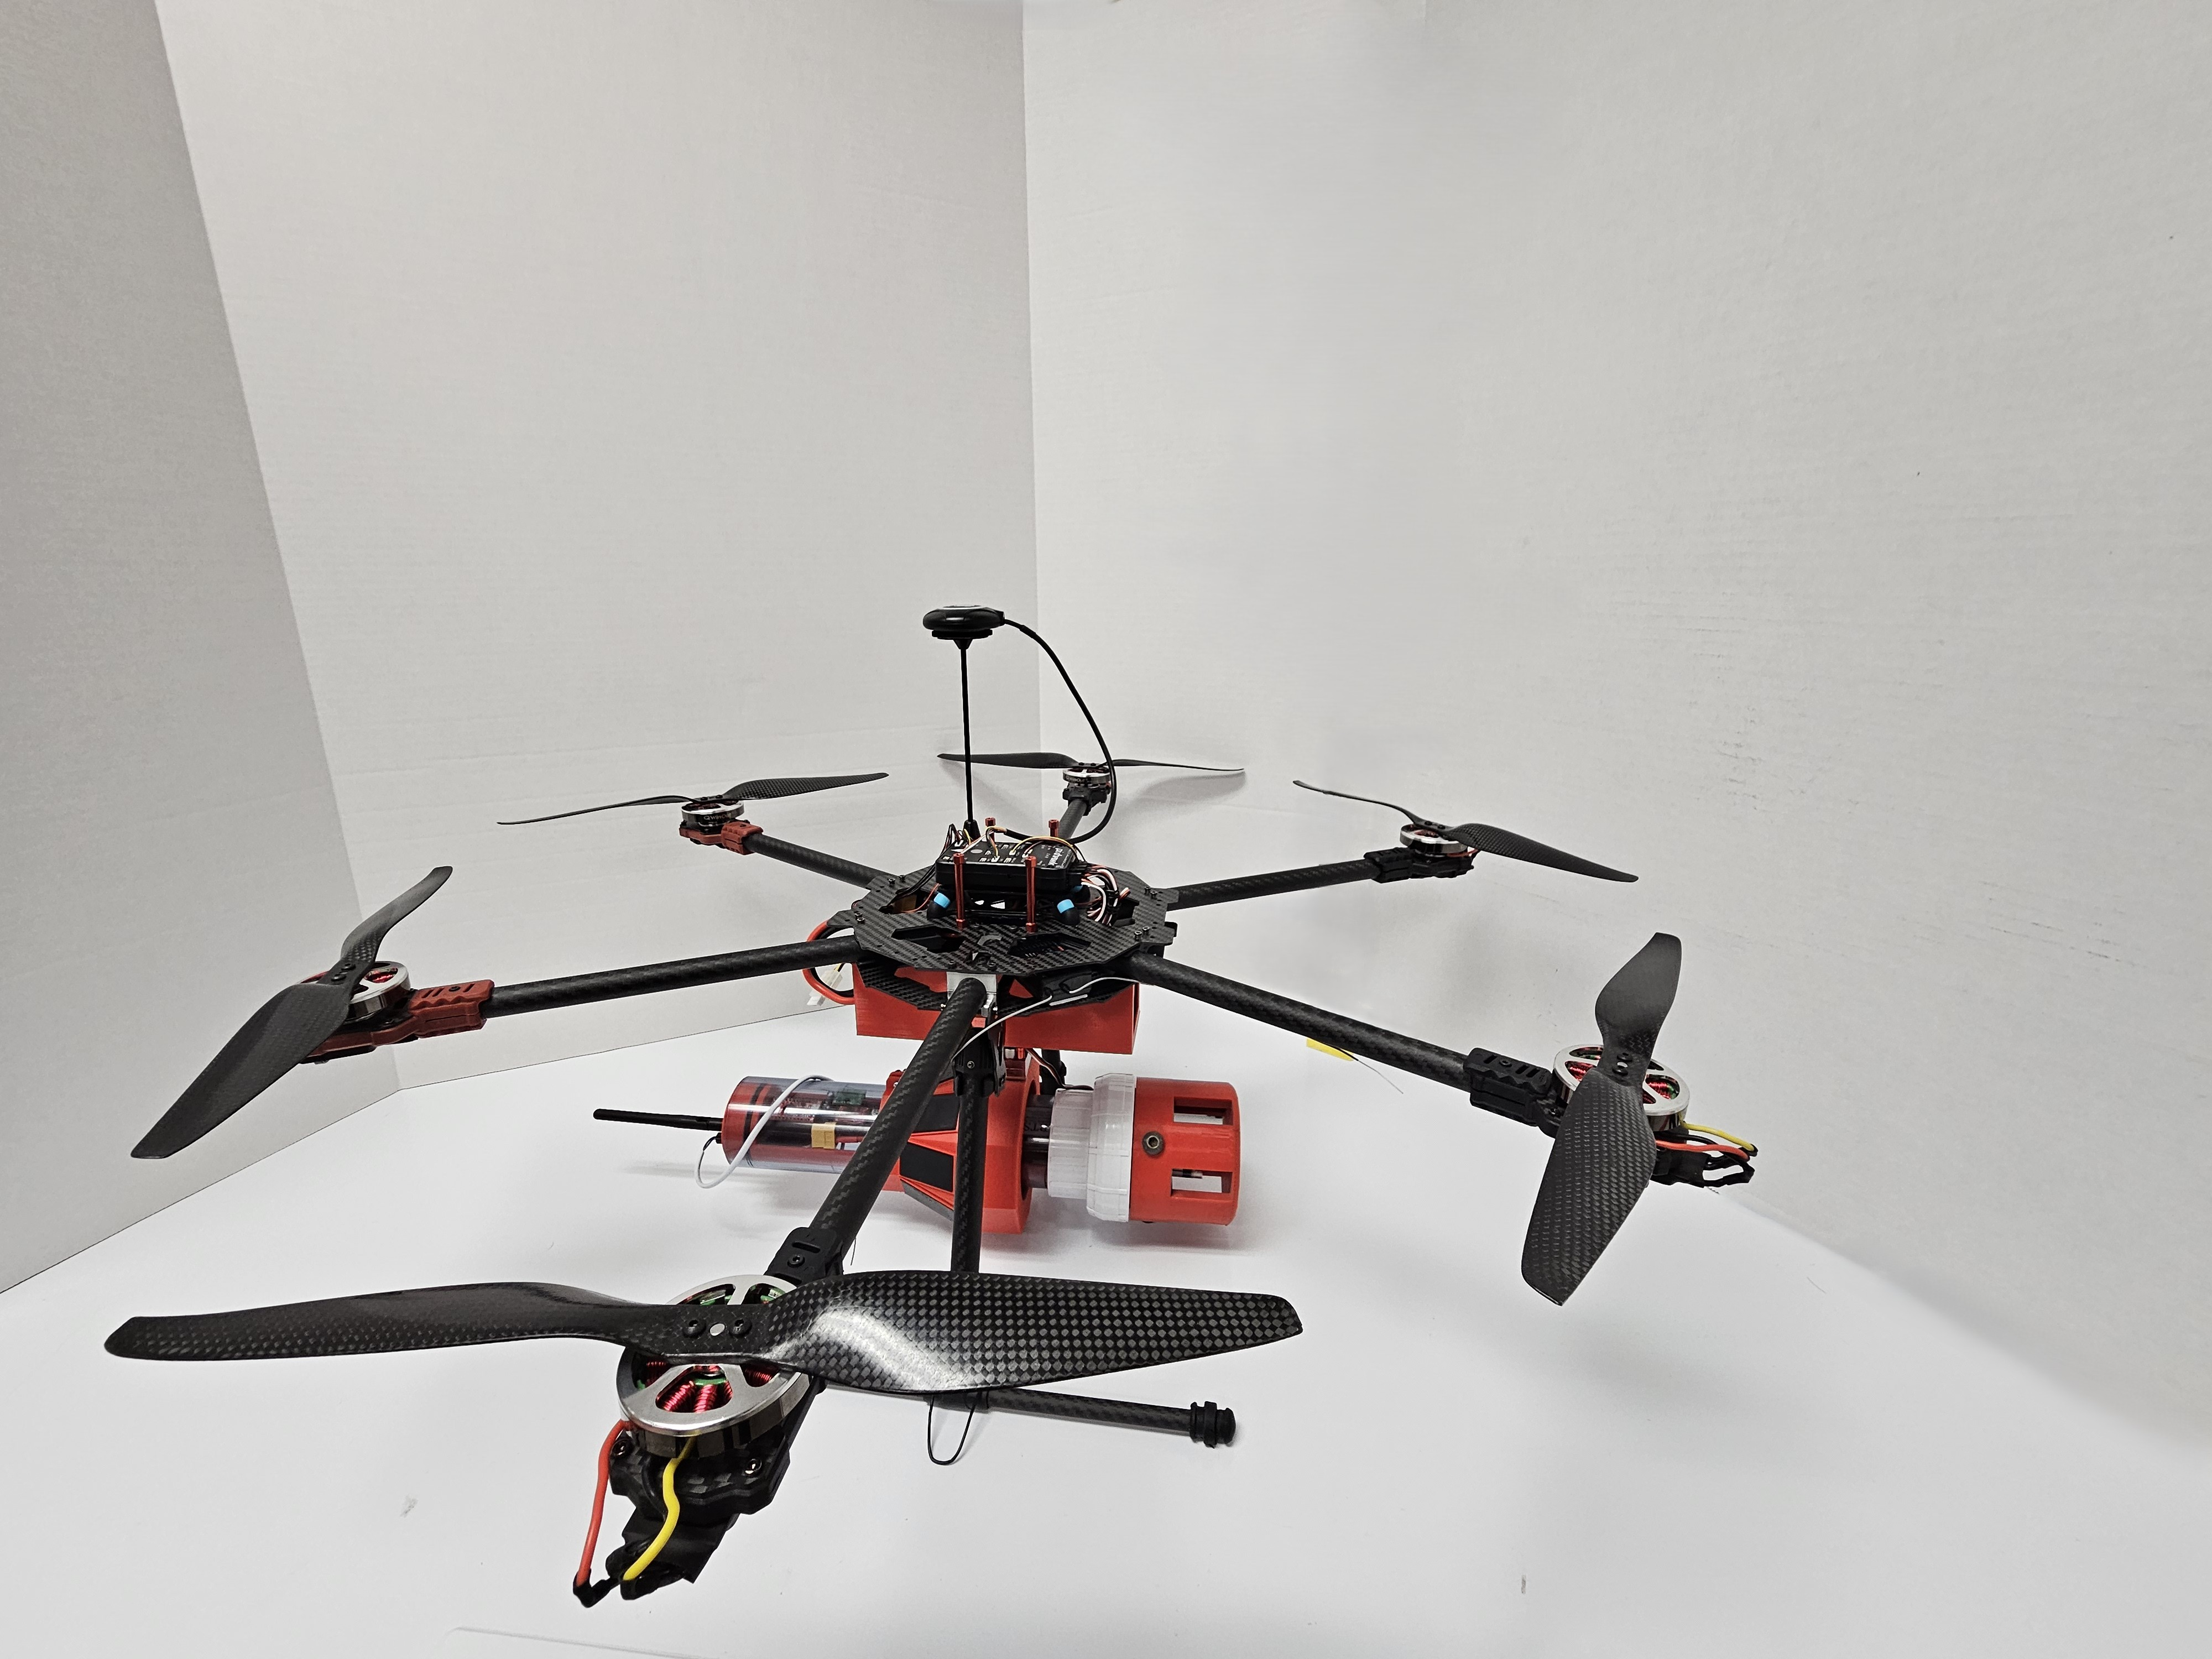
\includegraphics[width=5.0in]{figures/Figure1_Drone.jpg}
		\caption{Full drone setup showing main frame and propeller configuration.}
		\label{fig:Figure1_Drone}
	\end{figure}
	
	% Figure 2: EPM closeup
	\begin{figure}[H]
		\centering
		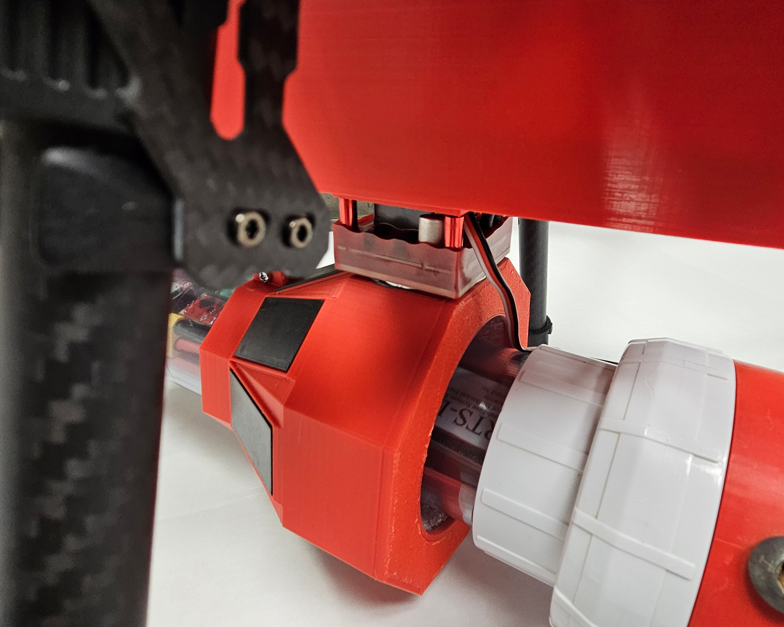
\includegraphics[width=4.5in]{figures/Figure2_EPM.png}
		\caption{Close-up of Electro-Permanent Magnet (EPM) attachment.}
		\label{fig:Figure2_EMP}
	\end{figure}
	
	
	\section{Analysis Figures}
	
	% Figure 3: 3D Trajectory
	\begin{figure}[H]
		\centering
		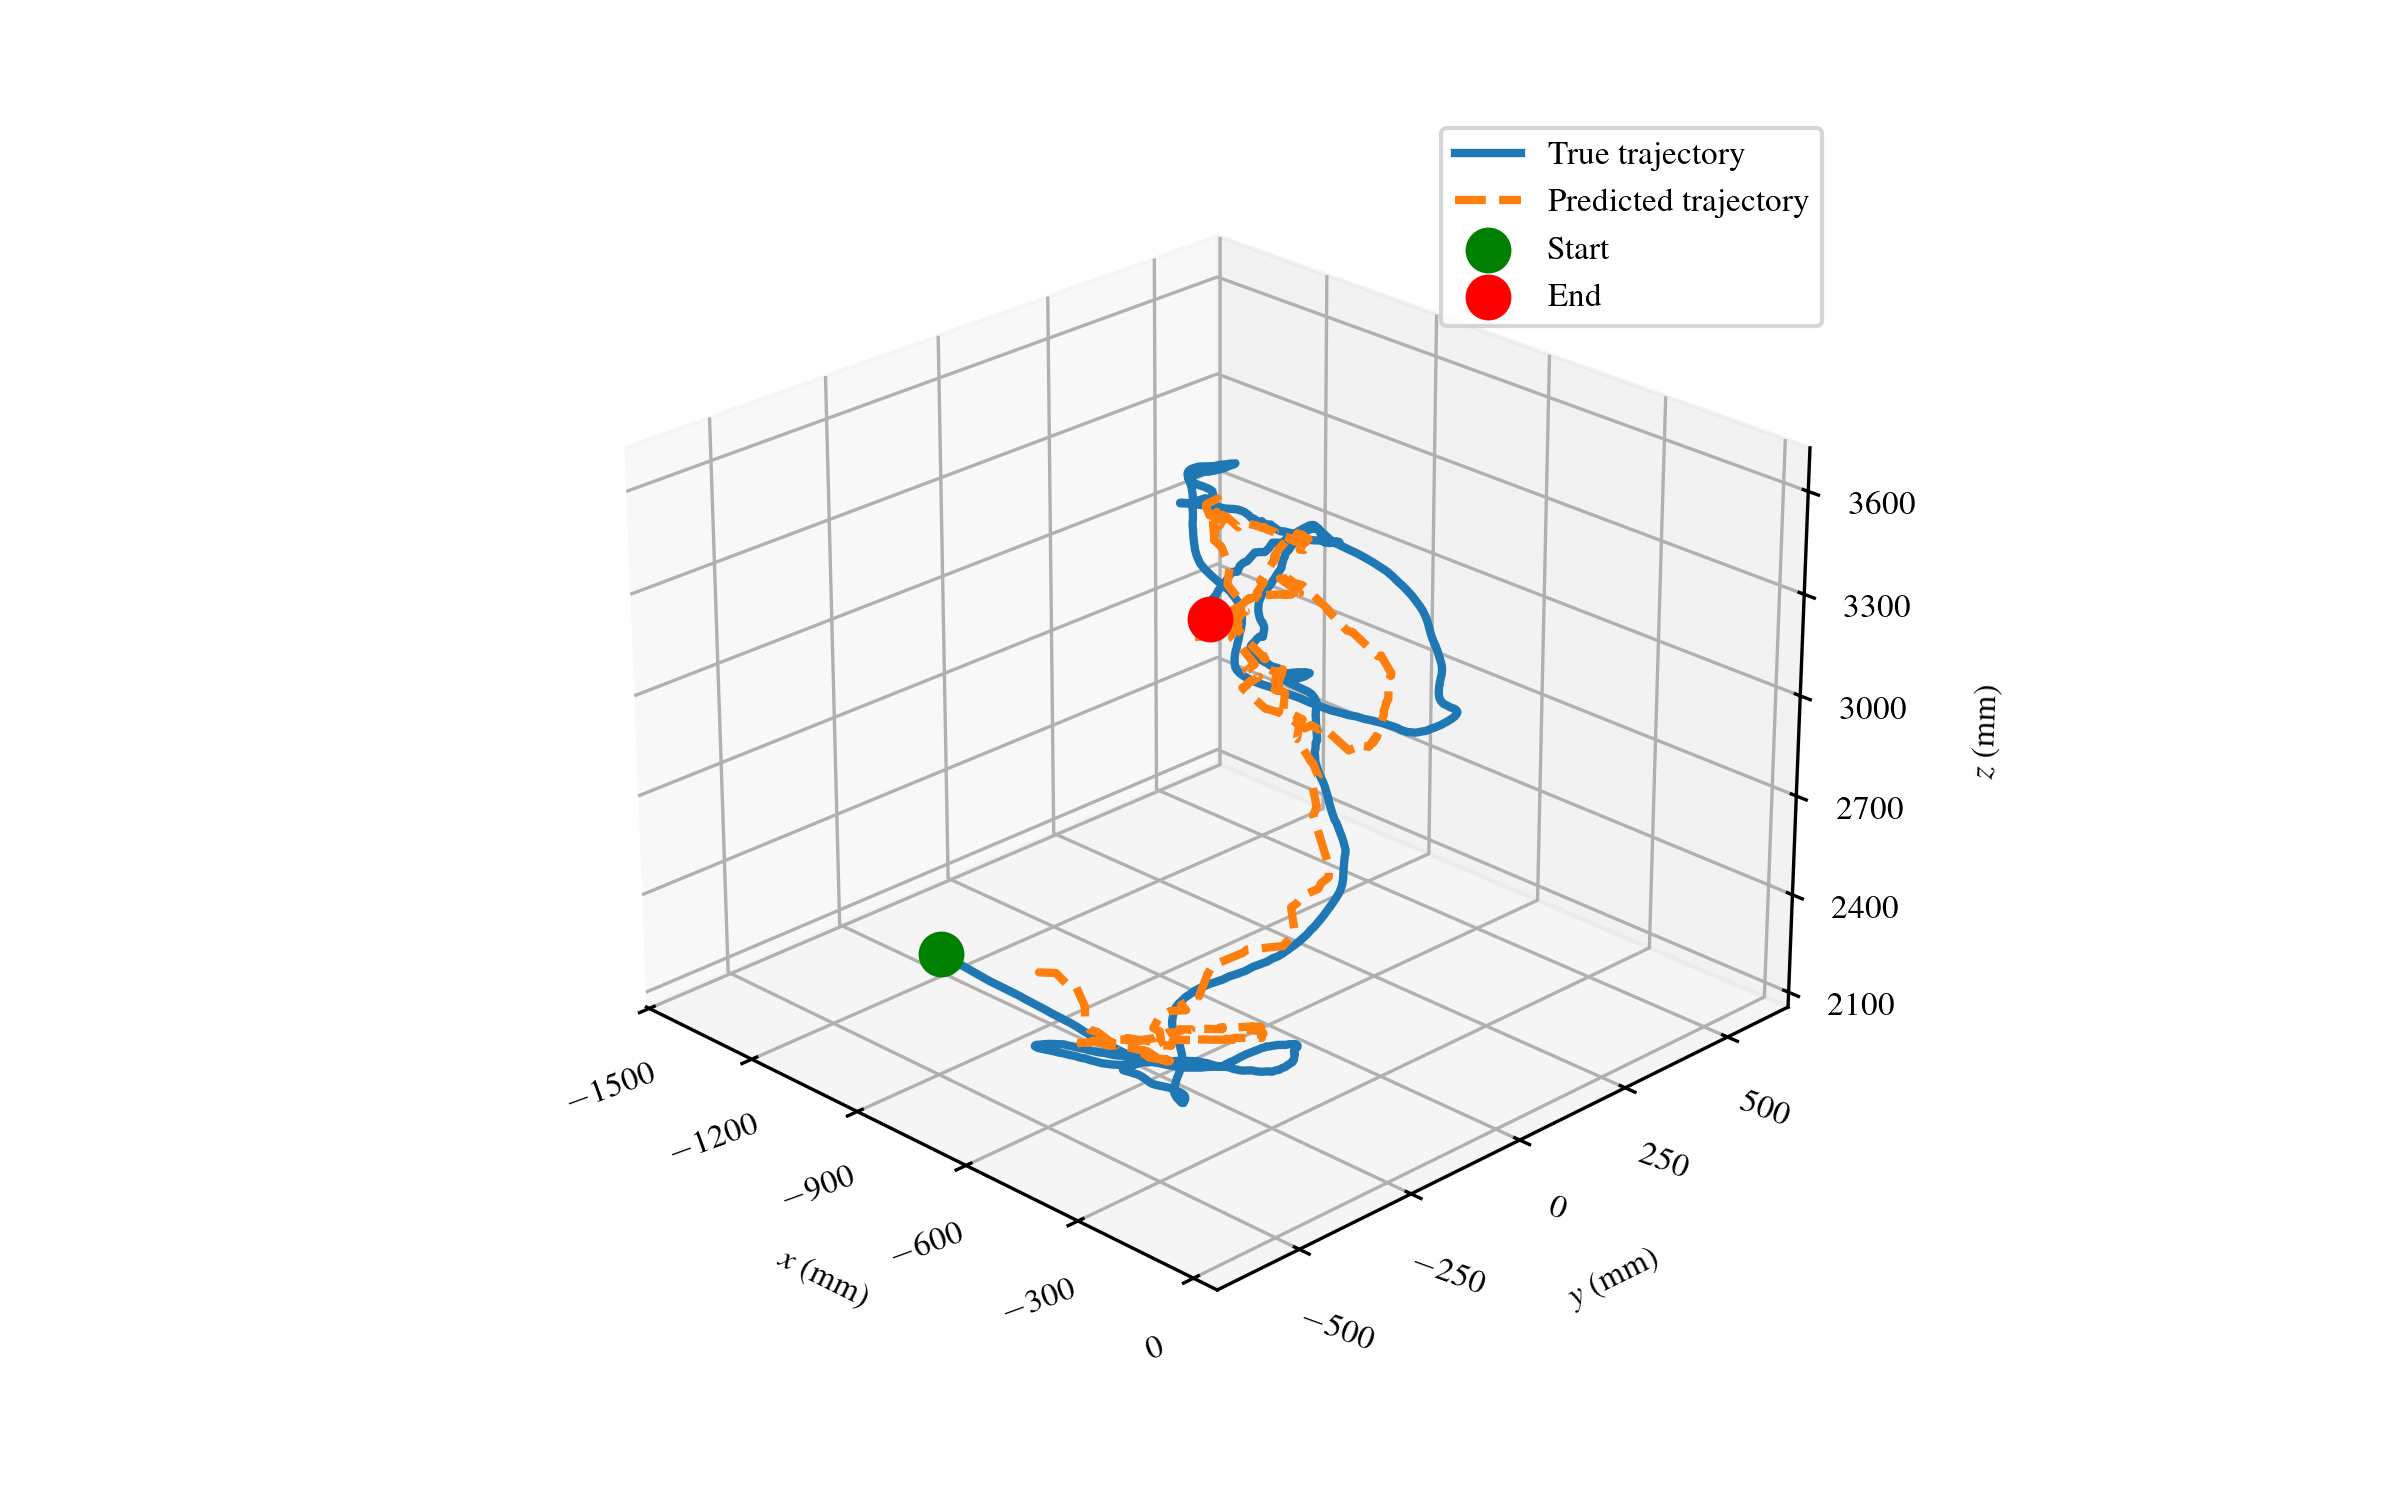
\includegraphics[width=6.0in]{figures/Figure3_3D_Trajectory.png}
		\caption{Comparison of the drone's 3D trajectory, showing predicted and true flight paths.}
		\label{fig:Figure3_3D_Trajectory}
	\end{figure}
	
	% Figure 4: Error Distribution
	\begin{figure}[H]
		\centering
		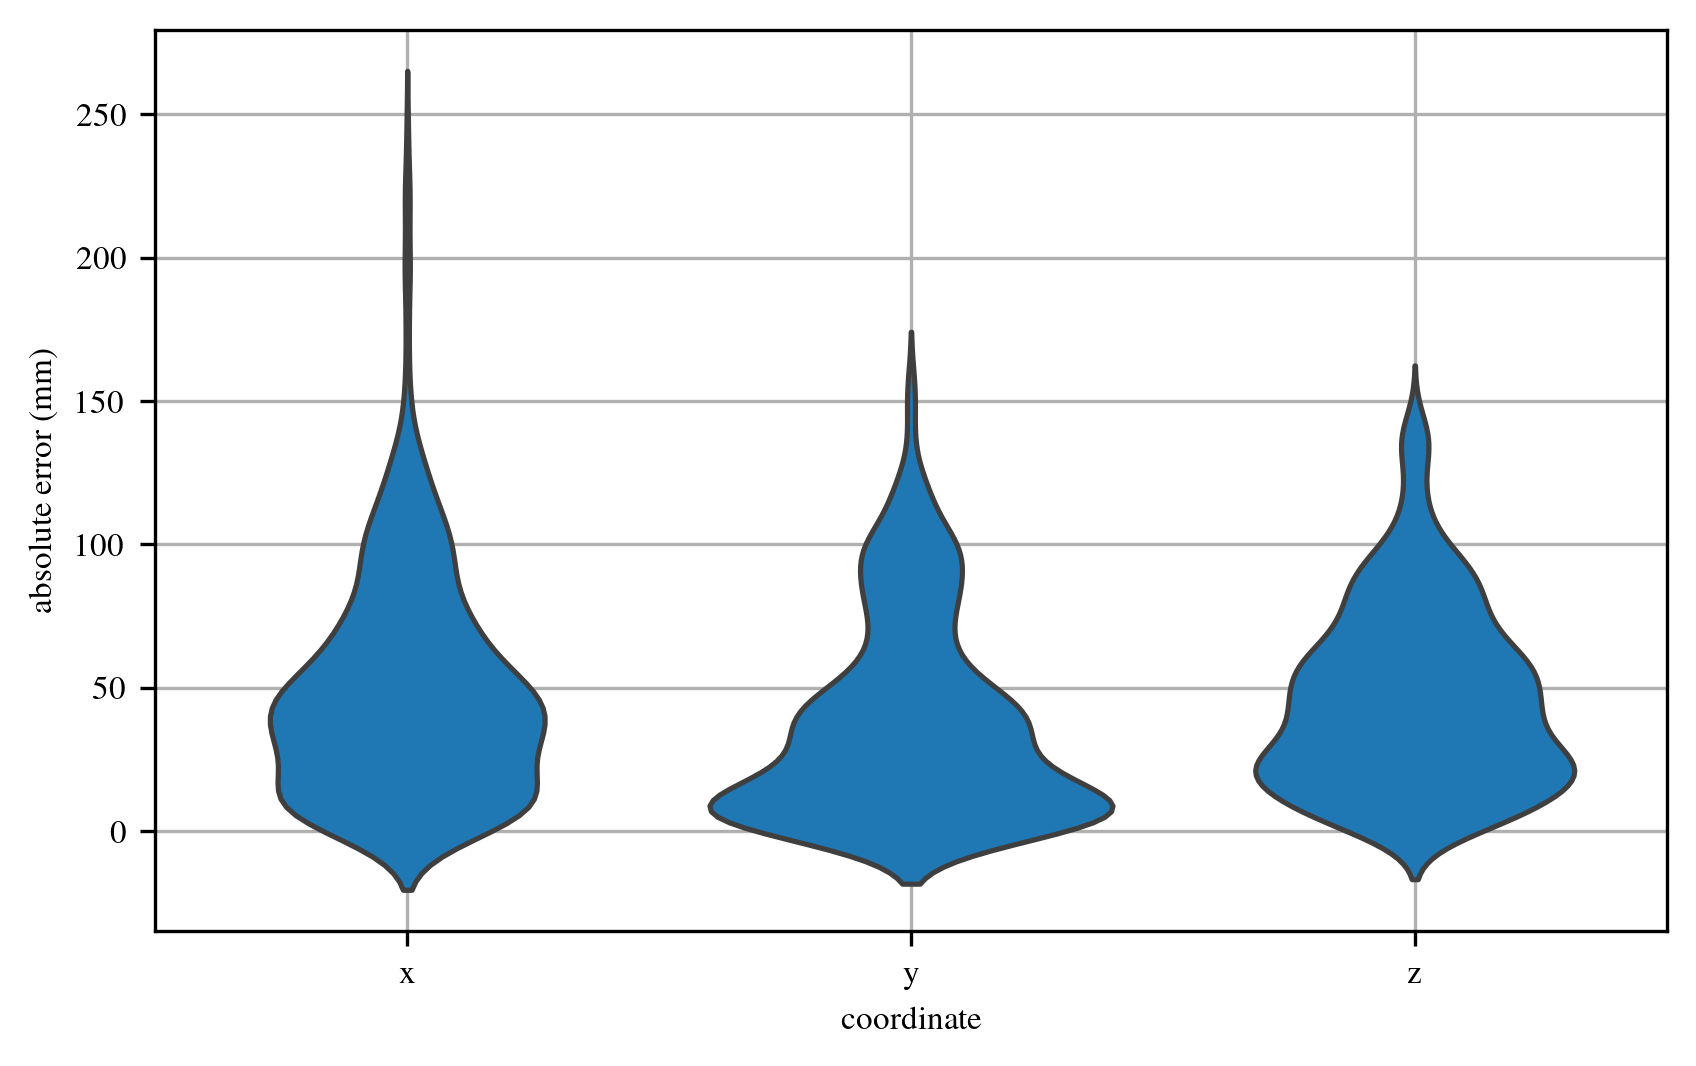
\includegraphics[width=6.0in]{figures/Figure4_Error_Distribution.png}
		\caption{Distribution of prediction errors for X, Y, and Z coordinates.}
		\label{fig:Figure4_Error_Distribution}
	\end{figure}
	
	% Figure 5: Scatter Plots
	\begin{figure}[H]
		\centering
		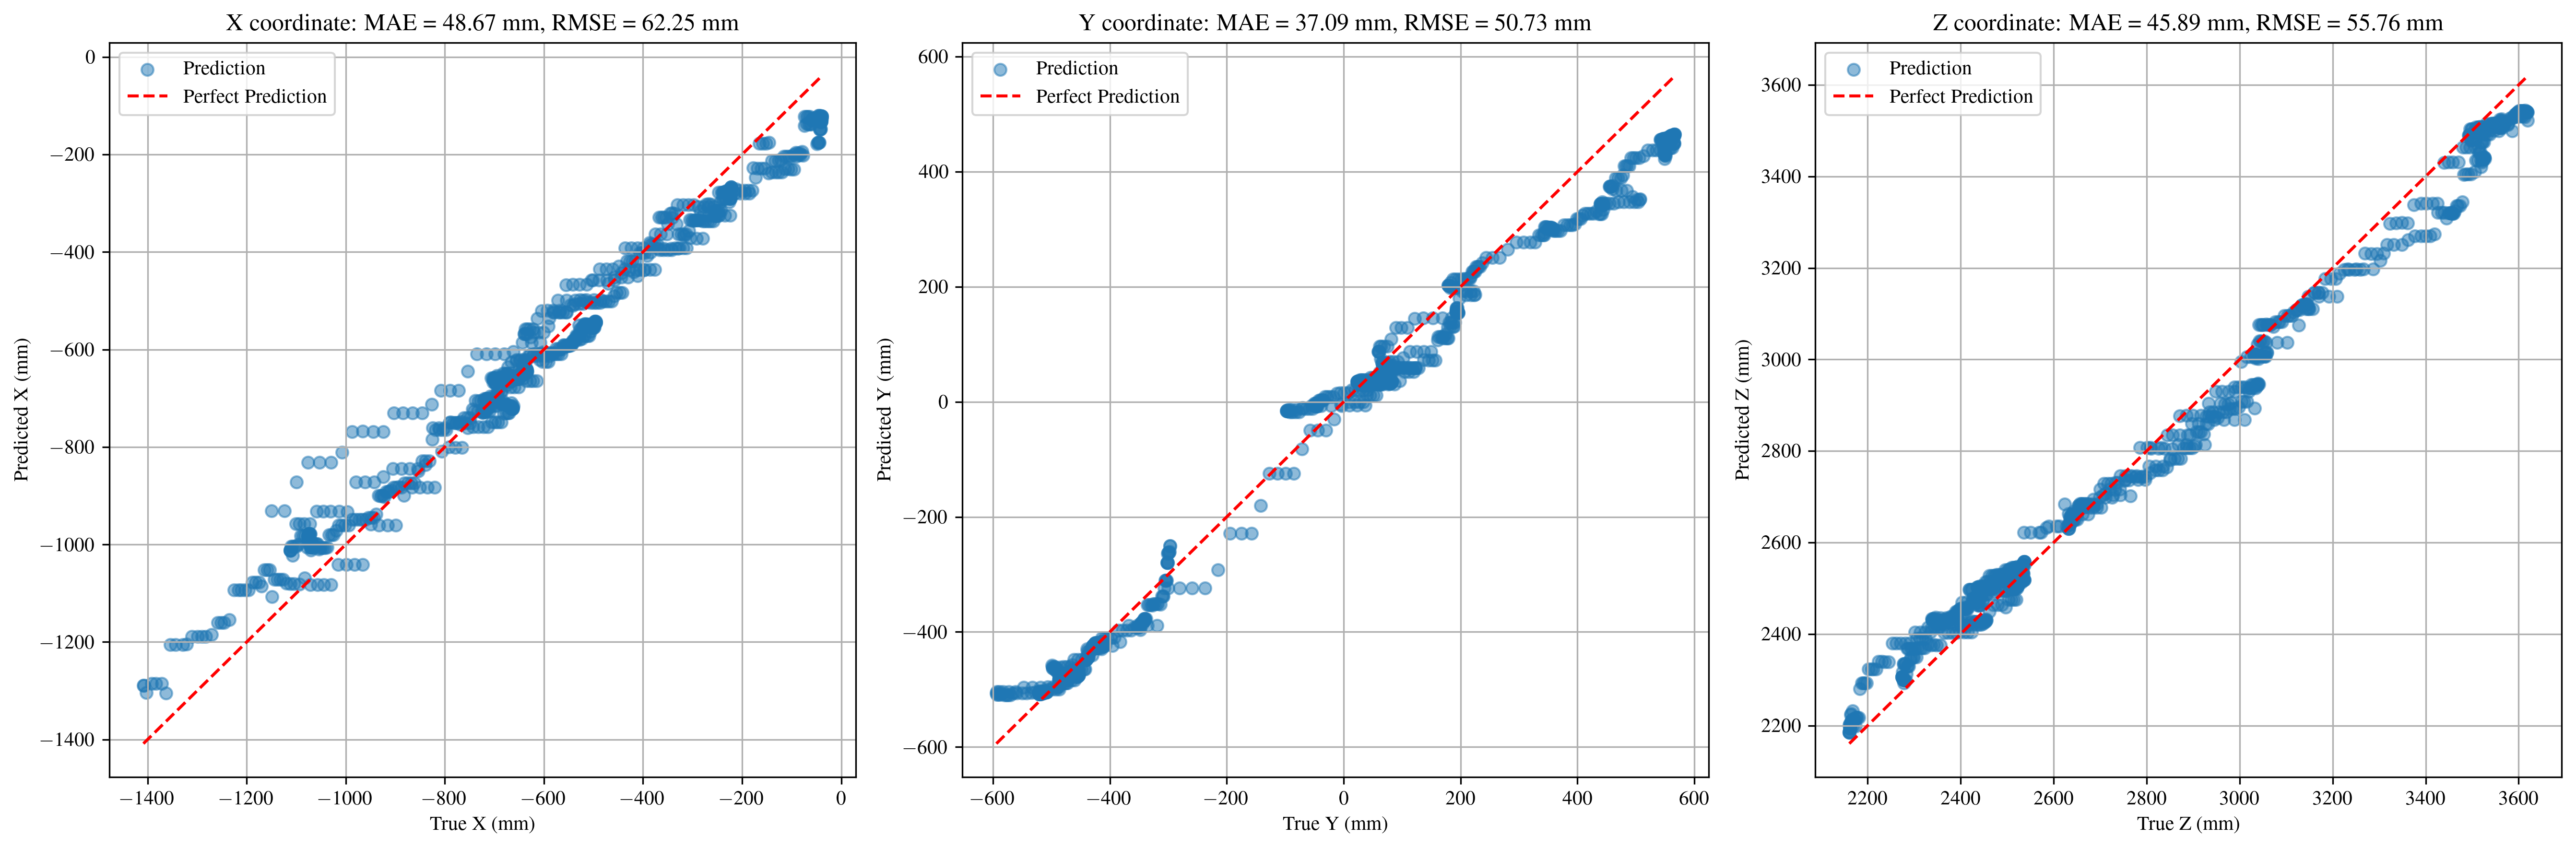
\includegraphics[width=6.5in]{figures/Figure5_Scatter_Plots.png}
		\caption{Scatter plots visualizing predicted versus true coordinates for X, Y, and Z.}
		\label{fig:Figure5_Scatter_Plots}
	\end{figure}
	
	% Figure 6: Error Over Time
	\begin{figure}[H]
		\centering
		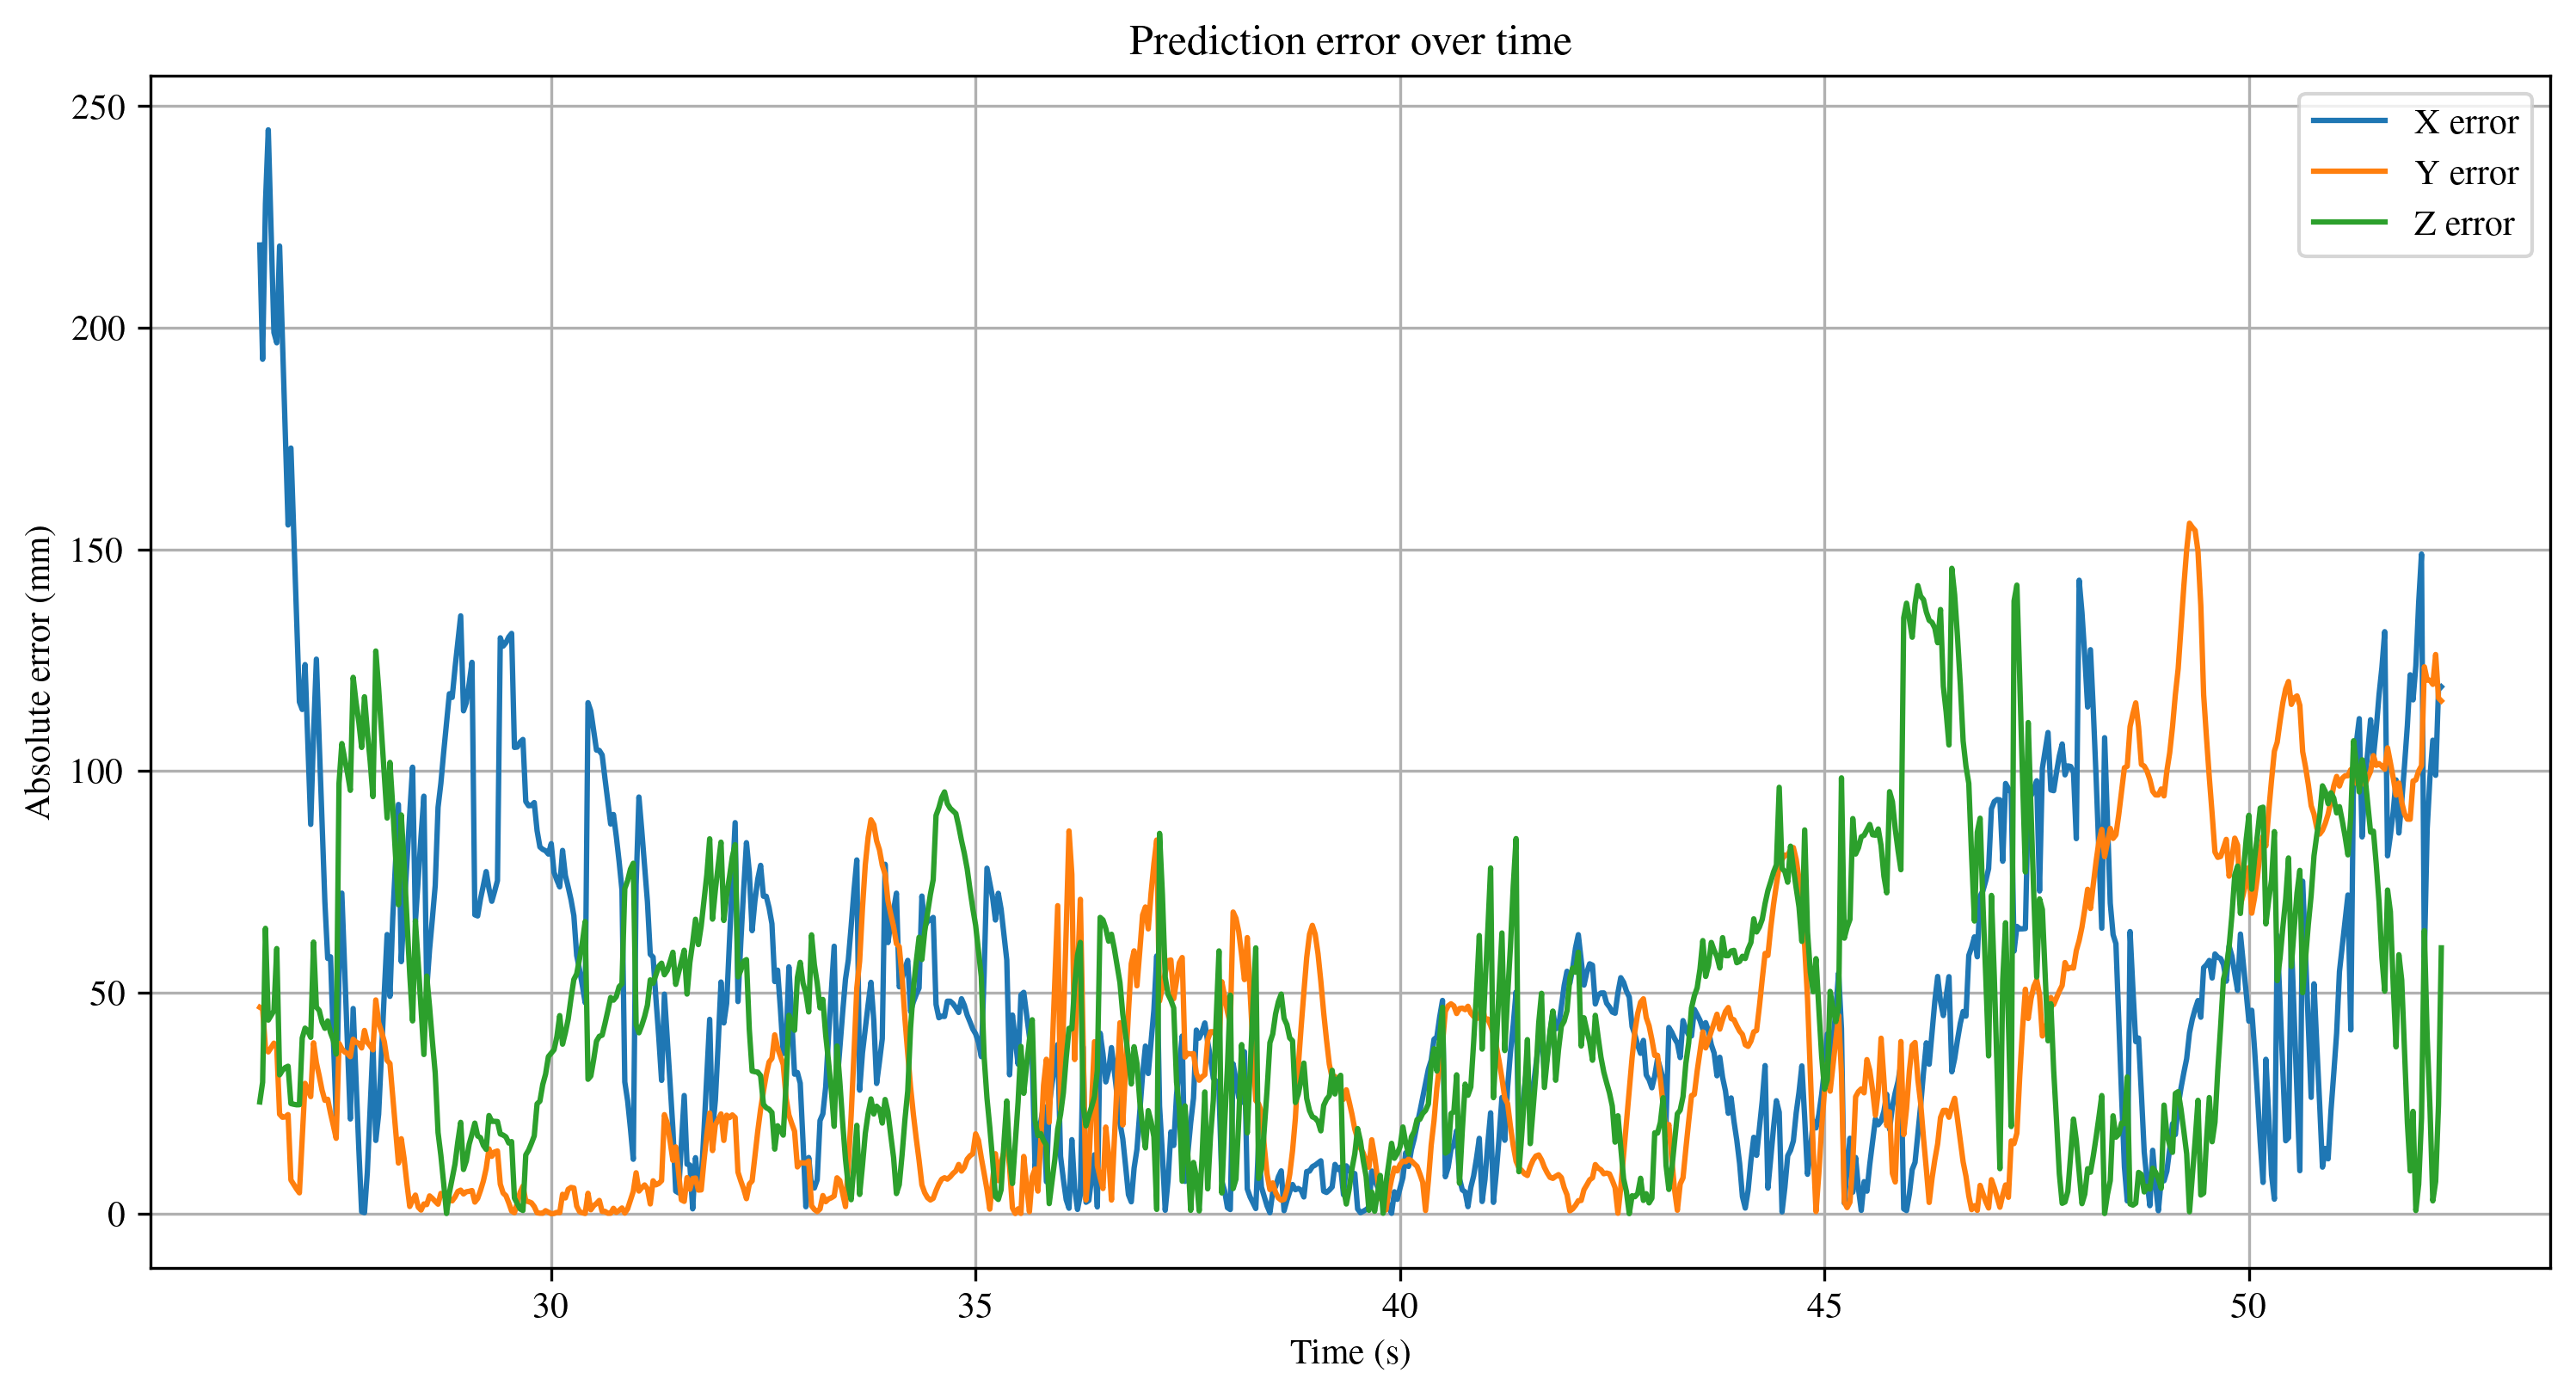
\includegraphics[width=6.5in]{figures/Figure6_Error_Over_Time.png}
		\caption{Prediction error visualized over time for each axis (X, Y, Z).}
		\label{fig:Figure6_Error_Over_Time}
	\end{figure}
	
\end{document}
